\documentclass[10pt,aspectratio=169]{beamer}

\usetheme{Madrid}
\usecolortheme{default}
\setbeamertemplate{navigation symbols}{}
\setbeamertemplate{footline}[frame number]

\usepackage{amsmath}
\usepackage{graphicx}
\usepackage{booktabs}
\usepackage{xcolor}

\graphicspath{{../mn_plots/}}

\title[Moment Networks]{Moment Networks}
\author{}
\date{\today}

\newcommand{\signal}{s}
\newcommand{\data}{d}
\newcommand{\synth}{s'}
\newcommand{\target}{\tilde{s}}
\newcommand{\noise}{n}
\newcommand{\net}{f_\theta}

\begin{document}

\begin{frame}
  \titlepage
\end{frame}

\begin{frame}{Goal}
  \begin{block}{What we want}
    For each Planck patch, use the data map \(\data\) to learn the posterior
    \[
      p(\signal \mid \data).
    \]

    We then want to use a NN to infer the first two moments:
    \[
      \mathbb{E}[\signal \mid \data],
      \qquad
      \operatorname{Std}[\signal \mid \data].
    \]
  \end{block}

  \vspace{0.4em}
  Here
  \[
    \signal =
    \begin{pmatrix}
      Q^{s} \\
      U^{s}
    \end{pmatrix},
    \qquad
    \data =
    \begin{pmatrix}
      Q^{d} \\
      U^{d}
    \end{pmatrix}.
  \]

  The output maps should have the original patch resolution, \(384 \times 384\).
\end{frame}

\begin{frame}{Basic Supervised Problem}
  We train on synthetic signal/data pairs:
  \[
    \data_i = \synth_i + \noise_i.
  \]

  \vspace{0.4em}
  \begin{itemize}
    \item \(\synth_i\): synthesized signal map from component-separated patch statistics.
    \item \(\noise_i\): nuisance realization for the same patch.
    \item \(\data_i\): simulated observed data map.
  \end{itemize}

  \vspace{0.4em}
  The network learns a conditional map
  \[
    \data \longmapsto \text{posterior moments of } \signal \mid \data.
  \]
\end{frame}

\begin{frame}{Dataset Generation}
  For each patch \(p\):

  \begin{enumerate}
    \item Start from the component-separated result
      \[
        \target_p = (\tilde{Q}_p, \tilde{U}_p).
      \]
    \item Synthesize maps \(\synth_{p,i}\) matching scattering statistics.
    \item Augment the synthesized maps.
    \item Add same-patch nuisance realizations.
  \end{enumerate}

  \vspace{0.4em}
  Current dataset scale:
  \[
    10 \text{ syntheses per patch}
    \times
    8 \text{ augmentations}
    =
    80 \text{ pairs per patch}.
  \]

  Files contain
  \[
    (\synth_Q, d_Q, \synth_U, d_U)
  \]
  for every generated pair.
\end{frame}

\begin{frame}{Synthesis and Boundary Conditions}
  The real Planck patches are not periodic:
  \[
    \texttt{pbc} = \texttt{False}.
  \]

  \vspace{0.5em}
  For augmentation, we synthesize larger periodic maps and crop back:

  \begin{center}
  \begin{tabular}{lll}
    \toprule
    Object & Shape & Boundary condition \\
    \midrule
    Component-separated target & \(384 \times 384\) & non-periodic \\
    Running synthesis & larger map & periodic \\
    Final training image & \(384 \times 384\) & center crop \\
    \bottomrule
  \end{tabular}
  \end{center}

  \vspace{0.5em}
  This avoids applying periodic translations directly to non-periodic observed patches.
\end{frame}

\begin{frame}{Moment Network Loss}
  The reference implementations train a Gaussian moment network:
  \[
    \net(\data) =
    \left(
      \mu_\theta(\data),
      \log \sigma_\theta^2(\data)
    \right).
  \]

  For training pairs \(\{(\data_i,\synth_i)\}_{i=1}^N\), first learn the posterior mean:
  \[
    \mathcal{L}_{\rm mean}
    =
    \frac{1}{N}
    \sum_{i=1}^{N}
    \left\|
      \synth_i - \mu_\theta(\data_i)
    \right\|_2^2 .
  \]

  Then learn mean and per-pixel marginal variance with the pixelwise Gaussian NLL:
  \[
    \mathcal{L}_{\rm NLL}
    =
    \frac{1}{2N|\Omega|}
    \sum_{i=1}^{N}
    \sum_{r \in \Omega}
    \left[
      \log \sigma_\theta^2(\data_i)_r
      +
      \frac{
        \left(\synth_{i,r} - \mu_\theta(\data_i)_r\right)^2
      }{
        \sigma_\theta^2(\data_i)_r
      }
    \right].
  \]

  \(\Omega\) is the pixel grid. This is a diagonal Gaussian approximation, so it does not learn the full spatial covariance.
\end{frame}

\begin{frame}{Why Did the Std Maps Collapse?}
  The mean is strongly supervised by channel-specific targets:
  \[
    \mu_Q(d) \approx \mathbb{E}[s_Q \mid d],
    \qquad
    \mu_U(d) \approx \mathbb{E}[s_U \mid d].
  \]

  \vspace{0.4em}
  The std is learned indirectly through residual statistics:
  \[
    \sigma^2(d)_r
    \quad\text{is driven by}\quad
    \left(s'_r-\mu(d)_r\right)^2 .
  \]

  \vspace{0.4em}
  In the joint network, Q and U shared the same latent representation:
  \[
    (Q^d,U^d)
    \longmapsto
    (\log\sigma_Q^2,\log\sigma_U^2).
  \]

  If the dominant residual patterns are common to Q and U, the variance heads can learn nearly the same uncertainty template.
\end{frame}

\begin{frame}{Degrees of Freedom}
  During training, the degrees of freedom are the neural-network weights:
  \[
    \theta.
  \]

  \vspace{0.5em}
  During inference, the patch is fixed and the network produces maps:
  \[
    \mu_\theta(\data) \in \mathbb{R}^{384 \times 384},
    \qquad
    \sigma_\theta(\data) \in \mathbb{R}^{384 \times 384}.
  \]

  \vspace{0.5em}
  For polarization, this is done separately for \(Q\) and \(U\).
\end{frame}

\begin{frame}{Previous Version: Joint Network}
  The first implementation trained one shared Q/U network:
  \[
    (Q^d, U^d)
    \longmapsto
    (\mu_Q, \mu_U, \log\sigma_Q^2, \log\sigma_U^2).
  \]

  \vspace{0.7em}
  This produced reasonable-looking posterior mean maps.

  \vspace{0.7em}
  But the uncertainty maps were suspicious:
  \[
    \sigma_Q(\data) \approx \sigma_U(\data)
  \]
  in morphology.

  \vspace{0.7em}
  The likely issue was architectural: Q and U shared the full U-Net trunk.
\end{frame}

\begin{frame}{Previous Version: Example Inference}
  \centering
  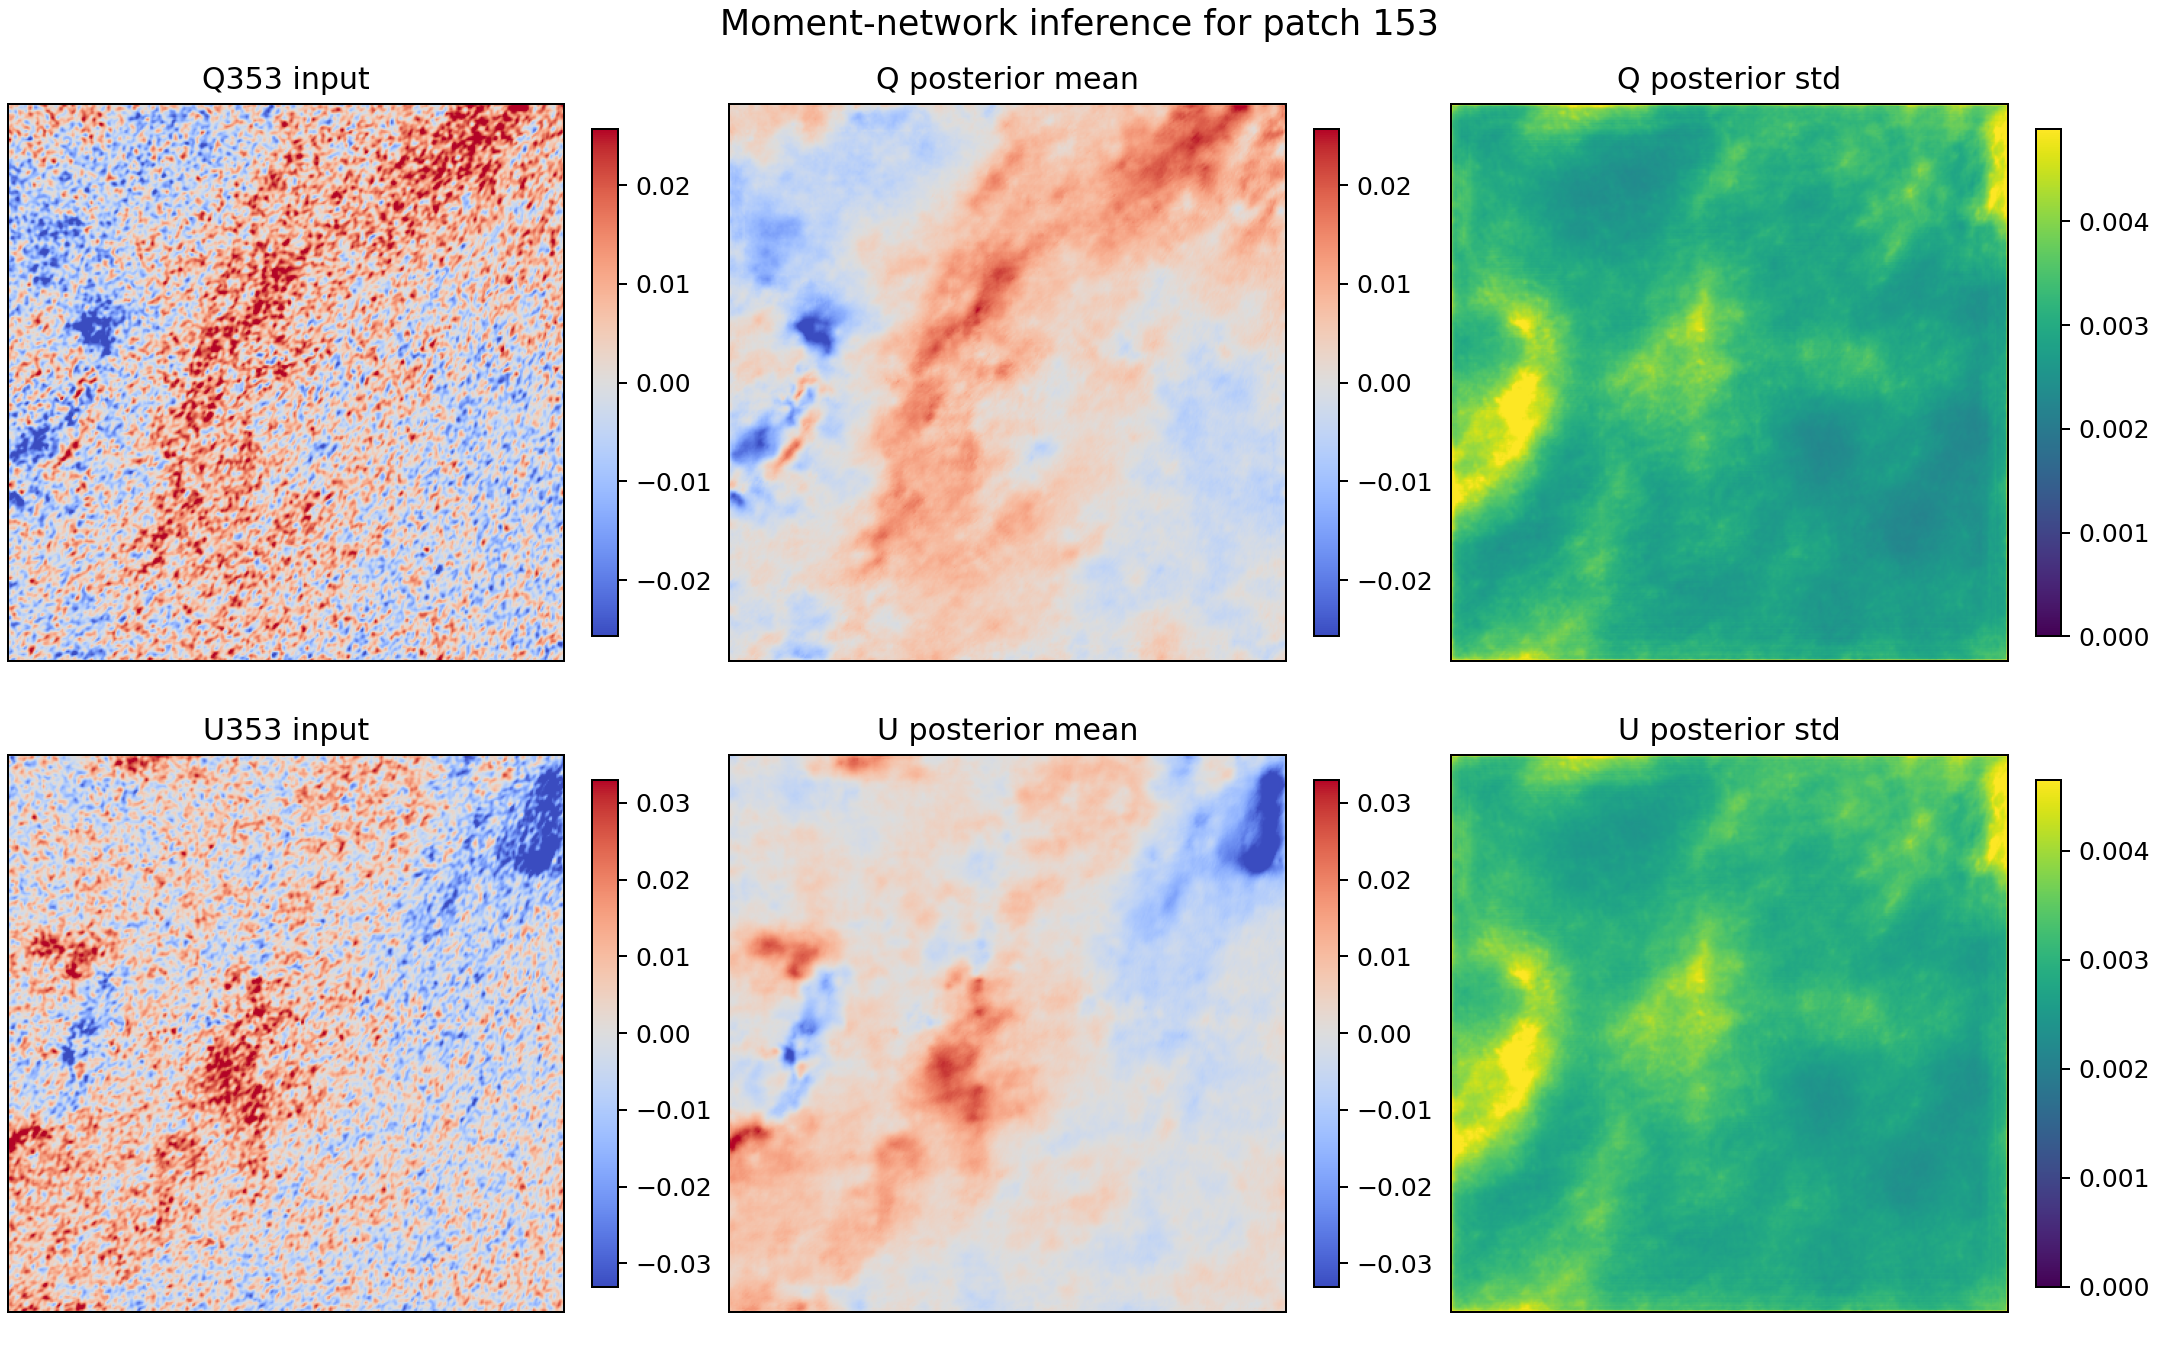
\includegraphics[height=0.72\textheight]{patch_153_moment_network_inference.png}

  \vspace{0.4em}
  \small
  Joint-network output for one patch. Mean maps look plausible, but Q/U uncertainty structure is too similar.
\end{frame}

\begin{frame}{Previous Version: Std Diagnostic}
  \centering
  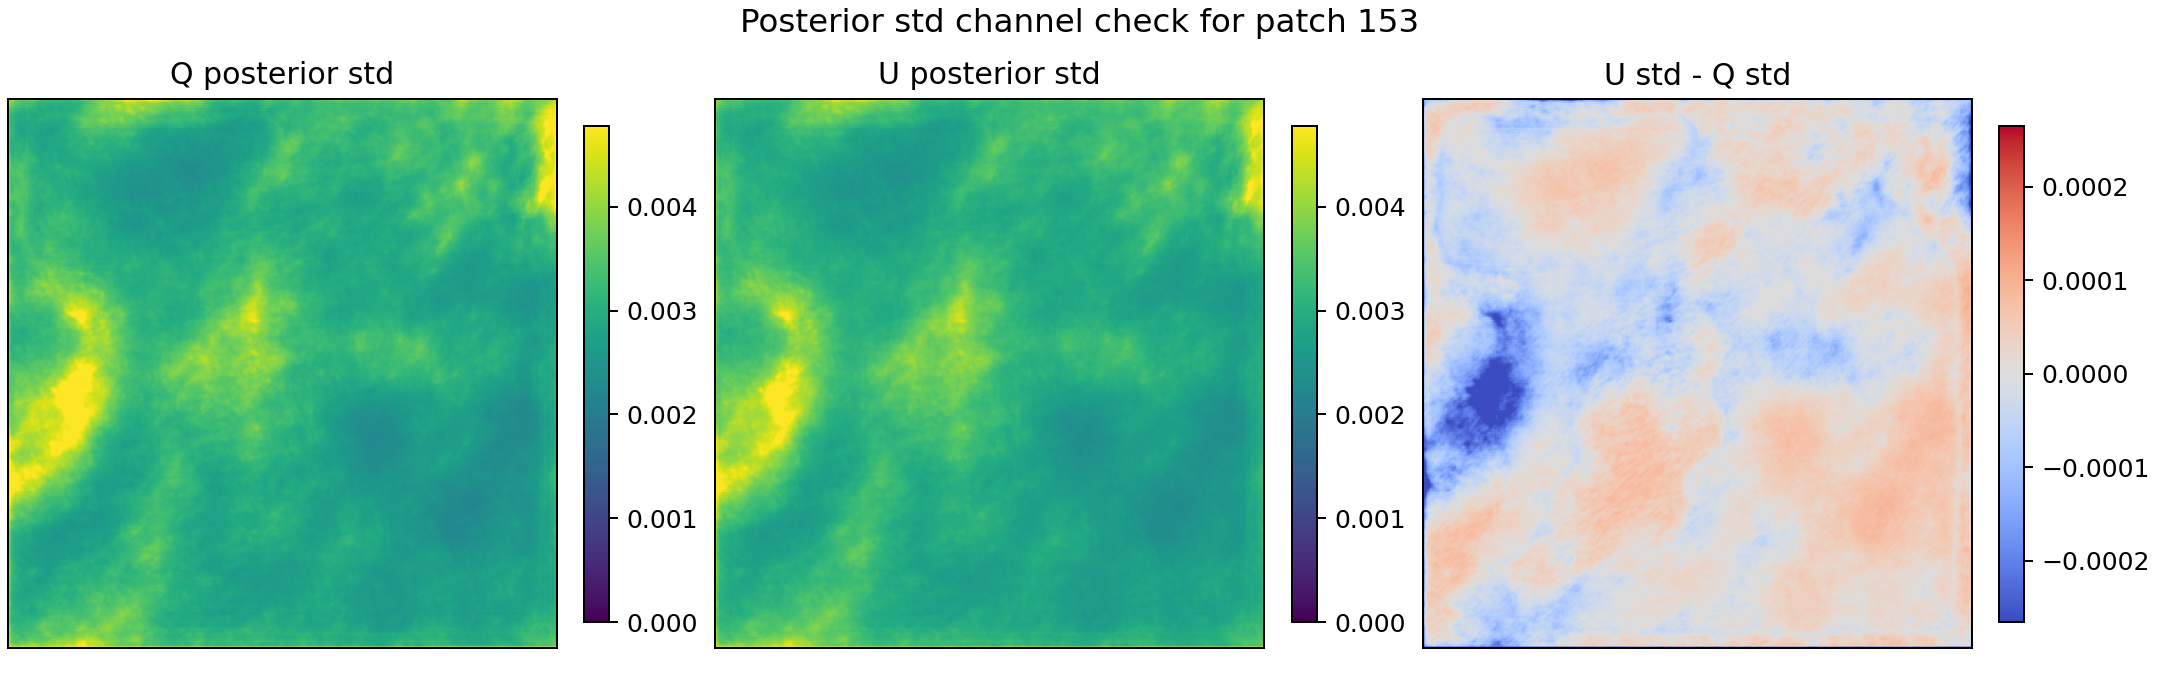
\includegraphics[width=0.78\linewidth,height=0.62\textheight,keepaspectratio]{patch_153_posterior_std_channel_check.png}

  \vspace{0.4em}
  \small
  The \(U\)-minus-\(Q\) std diagnostic exposed that the two std maps were close but not identical.
\end{frame}

\begin{frame}{New Algorithm: Inputs and Outputs}
  The current implementation uses intensity as an auxiliary input:
  \[
    \data =
    \begin{pmatrix}
      d_Q \\
      d_U \\
      d_I
    \end{pmatrix},
    \qquad
    \signal =
    \begin{pmatrix}
      s_Q \\
      s_U
    \end{pmatrix}.
  \]

  \vspace{0.5em}
  Here \(d_I\) is the downgraded \(I857\) map for the same patch.

  \vspace{0.5em}
  The network outputs posterior marginal moments:
  \[
    \data
    \longmapsto
    \left(
      \mu_Q,\ \mu_U,\ \sigma_Q,\ \sigma_U
    \right),
  \]
  where \(\sigma_Q\) and \(\sigma_U\) are per-pixel marginal posterior standard deviations.
\end{frame}

\begin{frame}{New Algorithm: Two Stages}
  We now train two U-Nets jointly over Q and U:

  \begin{center}
  \begin{tabular}{lll}
    \toprule
    Stage & Input & Output \\
    \midrule
    Mean network & \((d_Q,d_U,d_I)\) & \((\mu_Q,\mu_U)\) \\
    Variance network & \((d_Q,d_U,d_I)\) & \((\log\sigma_Q^2,\log\sigma_U^2)\) \\
    \bottomrule
  \end{tabular}
  \end{center}

  \vspace{0.7em}
  Stage 1 learns the conditional mean. Stage 2 freezes the mean network and learns the residual variance.
\end{frame}

\begin{frame}{New Algorithm: Mean Stage}
  For training pairs \(\{(\data_i,\synth_i)\}_{i=1}^N\), the mean network is
  \[
    m_\theta(\data_i)
    =
    \begin{pmatrix}
      \mu_Q(\data_i) \\
      \mu_U(\data_i)
    \end{pmatrix}.
  \]

  \vspace{0.5em}
  It is trained with
  \[
    \mathcal{L}_{\rm mean}
    =
    \frac{1}{N|\Omega|}
    \sum_{i=1}^{N}
    \sum_{r\in\Omega}
    \left\|
      \synth_{i,r} - m_\theta(\data_i)_r
    \right\|_2^2 .
  \]

  \vspace{0.5em}
  This estimates the posterior mean
  \[
    m_\theta(\data)
    \approx
    \mathbb{E}[\signal\mid\data].
  \]
\end{frame}

\begin{frame}{New Algorithm: Variance Stage}
  After training \(m_\theta\), we freeze it and form residual targets:
  \[
    \rho_i(r)
    =
    \log
    \left[
      \left(
        \synth_i(r) - m_\theta(\data_i)(r)
      \right)^2
      + \epsilon
    \right].
  \]

  \vspace{0.5em}
  The variance network \(v_\phi\) predicts
  \[
    v_\phi(\data)
    =
    \begin{pmatrix}
      \log\sigma_Q^2(\data) \\
      \log\sigma_U^2(\data)
    \end{pmatrix}.
  \]

  \vspace{0.5em}
  It minimizes
  \[
    \mathcal{L}_{\rm var}
    =
    \frac{1}{N|\Omega|}
    \sum_{i=1}^{N}
    \sum_{r\in\Omega}
    \left\|
      v_\phi(\data_i)_r - \rho_i(r)
    \right\|_2^2 .
  \]
\end{frame}

\begin{frame}{Current Implementation: Architecture}
  Both stages use the same small U-Net architecture:

  \vspace{0.4em}
  \begin{center}
  \begin{tabular}{lll}
    \toprule
    Network & Input channels & Output channels \\
    \midrule
    Mean U-Net & \(d_Q,d_U,d_I\) & \(\mu_Q,\mu_U\) \\
    Variance U-Net & \(d_Q,d_U,d_I\) & \(\log\sigma_Q^2,\log\sigma_U^2\) \\
    \bottomrule
  \end{tabular}
  \end{center}

  \vspace{0.5em}
  High-level structure:
  \[
    3 \rightarrow 16 \rightarrow 32 \rightarrow 64 \rightarrow 64
    \rightarrow 64 \rightarrow 32 \rightarrow 16 \rightarrow 2 .
  \]

  \vspace{0.4em}
  Downsampling uses average pooling; upsampling uses nearest-neighbor interpolation.
  Skip connections concatenate encoder and decoder features at matching resolution.
\end{frame}

\begin{frame}{Current Implementation: Normalization}
  Inputs and targets are normalized channel by channel before training:
  \[
    \widehat{\data}_{c}
    =
    \frac{\data_c-\bar{\data}_c}{\sigma_{\data,c}},
    \qquad
    \widehat{\signal}_{c}
    =
    \frac{\signal_c-\bar{\signal}_c}{\sigma_{\signal,c}} .
  \]

  \vspace{0.5em}
  The input channels are
  \[
    \data=(d_Q,d_U,d_I),
  \]
  and the target channels are
  \[
    \signal=(s_Q,s_U).
  \]

  \vspace{0.5em}
  The means and standard deviations are computed over the training split:
  \[
    \{(\data_i,\synth_i)\}_{i\in \mathcal{T}},
  \]
  using all pixels and all augmented samples. They are saved with the model checkpoint and reused at inference.
\end{frame}

\begin{frame}{Current Implementation: Why Normalize?}
  The Q, U, and \(I857\) channels have different numerical scales.

  \vspace{0.5em}
  Normalization makes the optimization problem better conditioned:
  \[
    (d_Q,d_U,d_I)
    \longrightarrow
    (\widehat{d}_Q,\widehat{d}_U,\widehat{d}_I).
  \]

  \vspace{0.5em}
  The network predicts moments in normalized target units:
  \[
    \widehat{\mu}_Q,\widehat{\mu}_U,
    \qquad
    \log \widehat{\sigma}_Q^2,\log \widehat{\sigma}_U^2.
  \]

  \vspace{0.5em}
  At inference, we transform back:
  \[
    \mu_c
    =
    \sigma_{\signal,c}\widehat{\mu}_c+\bar{\signal}_c,
    \qquad
    \sigma_c
    =
    \sigma_{\signal,c}\widehat{\sigma}_c.
  \]
\end{frame}

\begin{frame}{New Algorithm: Inference}
  For a selected patch:

  \begin{enumerate}
    \item Load observed maps:
      \[
        Q_{768}, U_{768}, I857_{768}.
      \]
    \item Downgrade by \(2\times2\) block averaging:
      \[
        d_Q,d_U,d_I \in \mathbb{R}^{384 \times 384}.
      \]
    \item Run the mean network and variance network.
  \end{enumerate}

  \vspace{0.4em}
  Final products:
  \[
    \mu_Q,\ \sigma_Q,\ \mu_U,\ \sigma_U.
  \]
\end{frame}

\begin{frame}{Previous Version: More Examples}
  \centering
  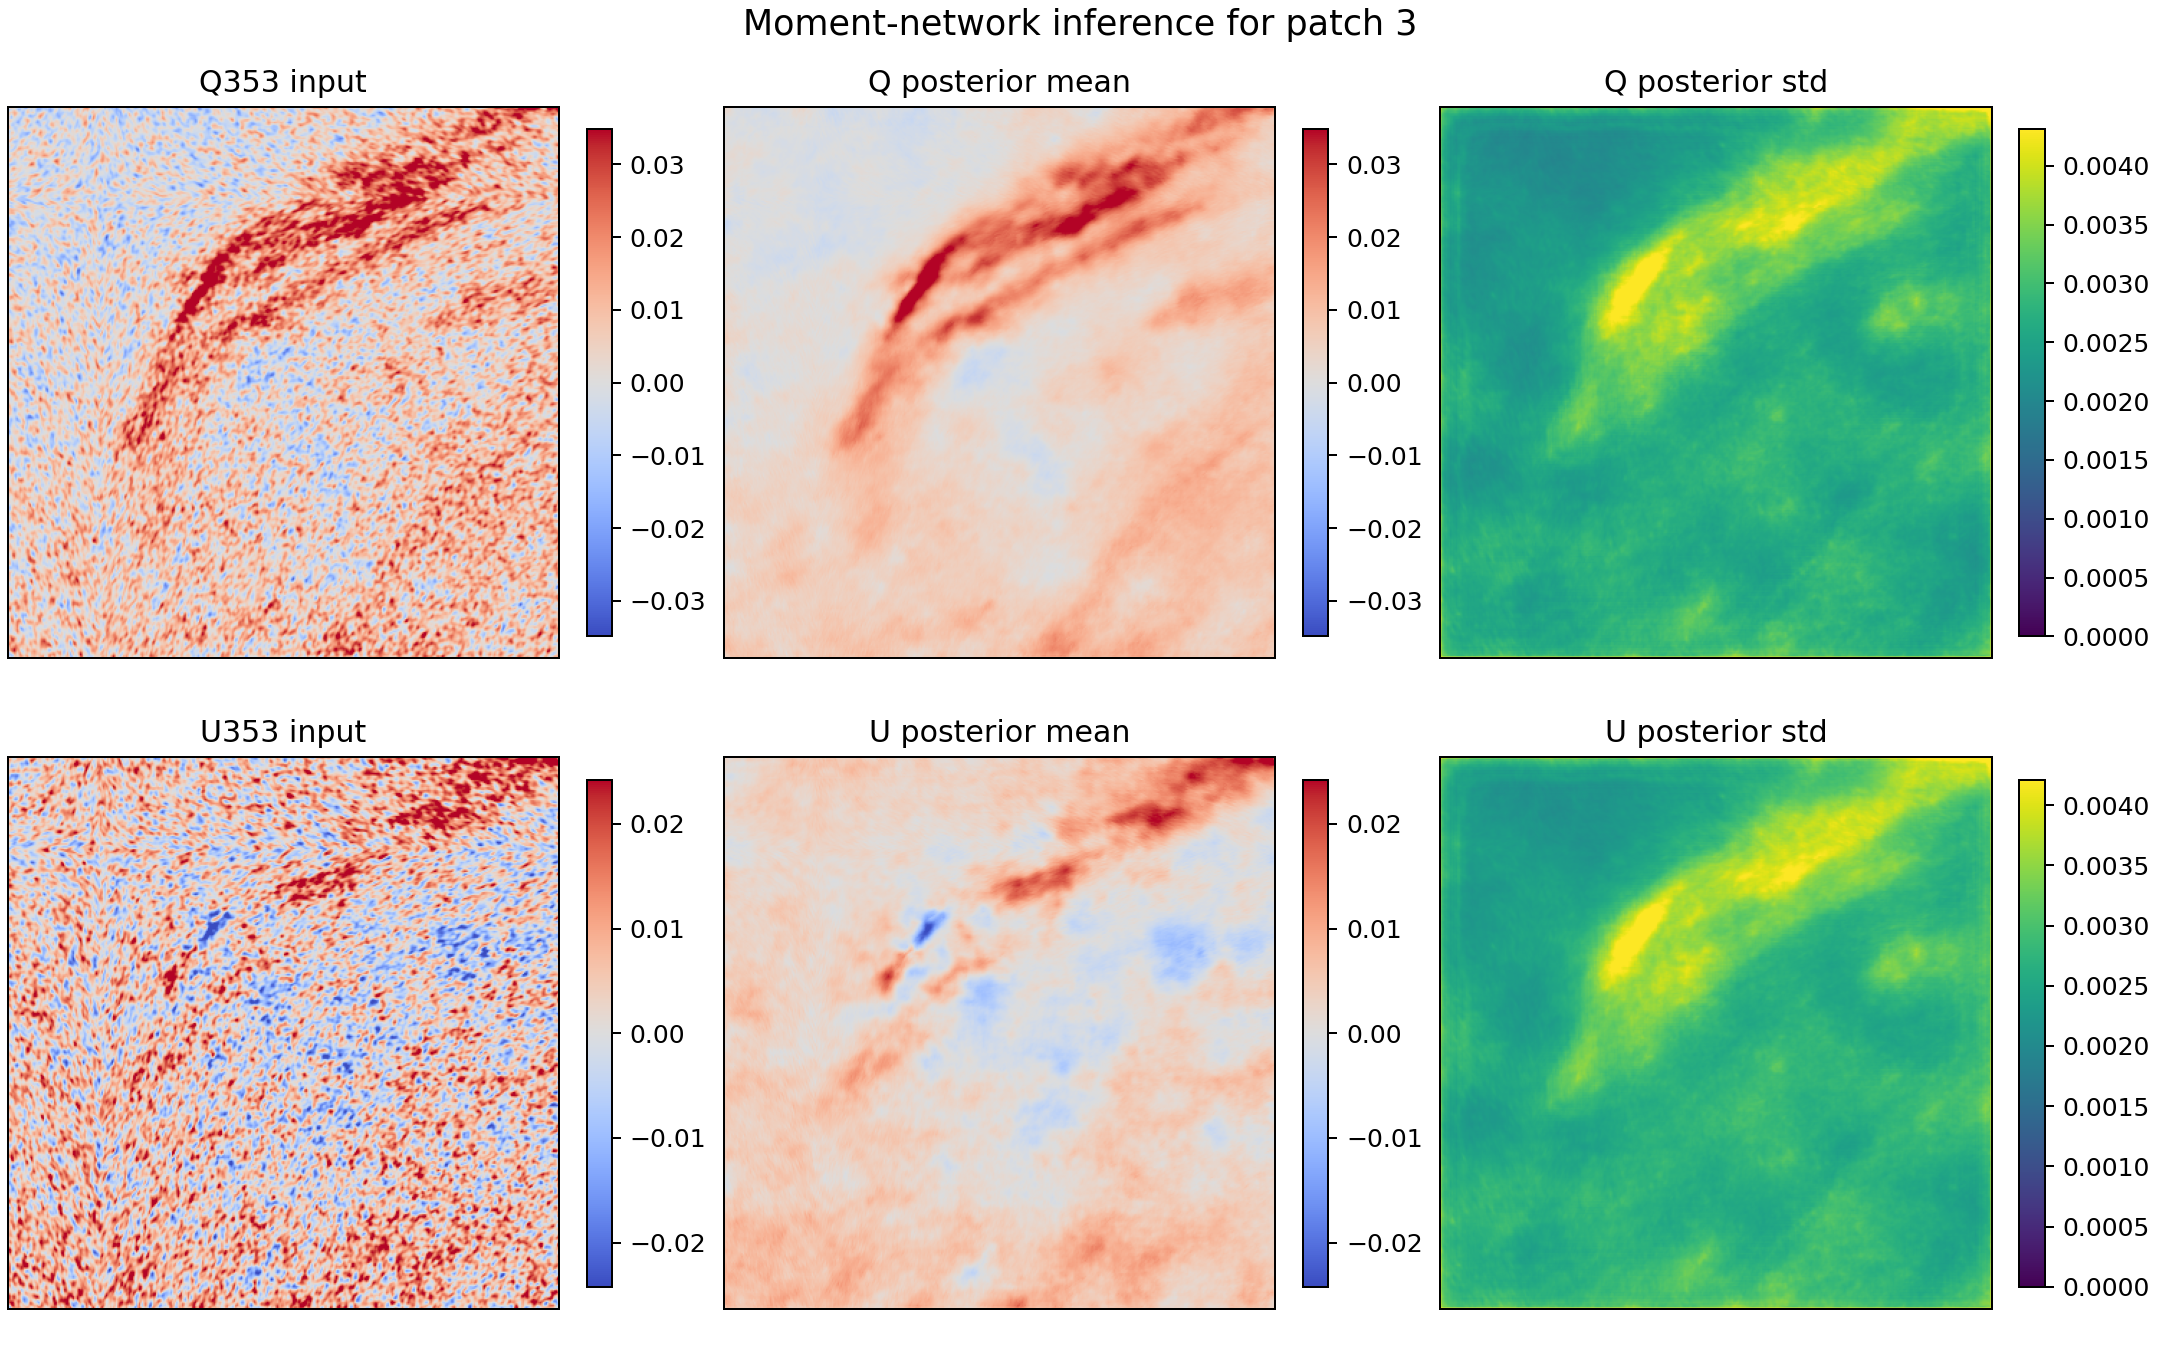
\includegraphics[height=0.72\textheight]{patch_3_moment_network_inference.png}

  \vspace{0.4em}
  \small
  Example from the previous joint-network run.
\end{frame}

\begin{frame}{Previous Version: More Examples}
  \centering
  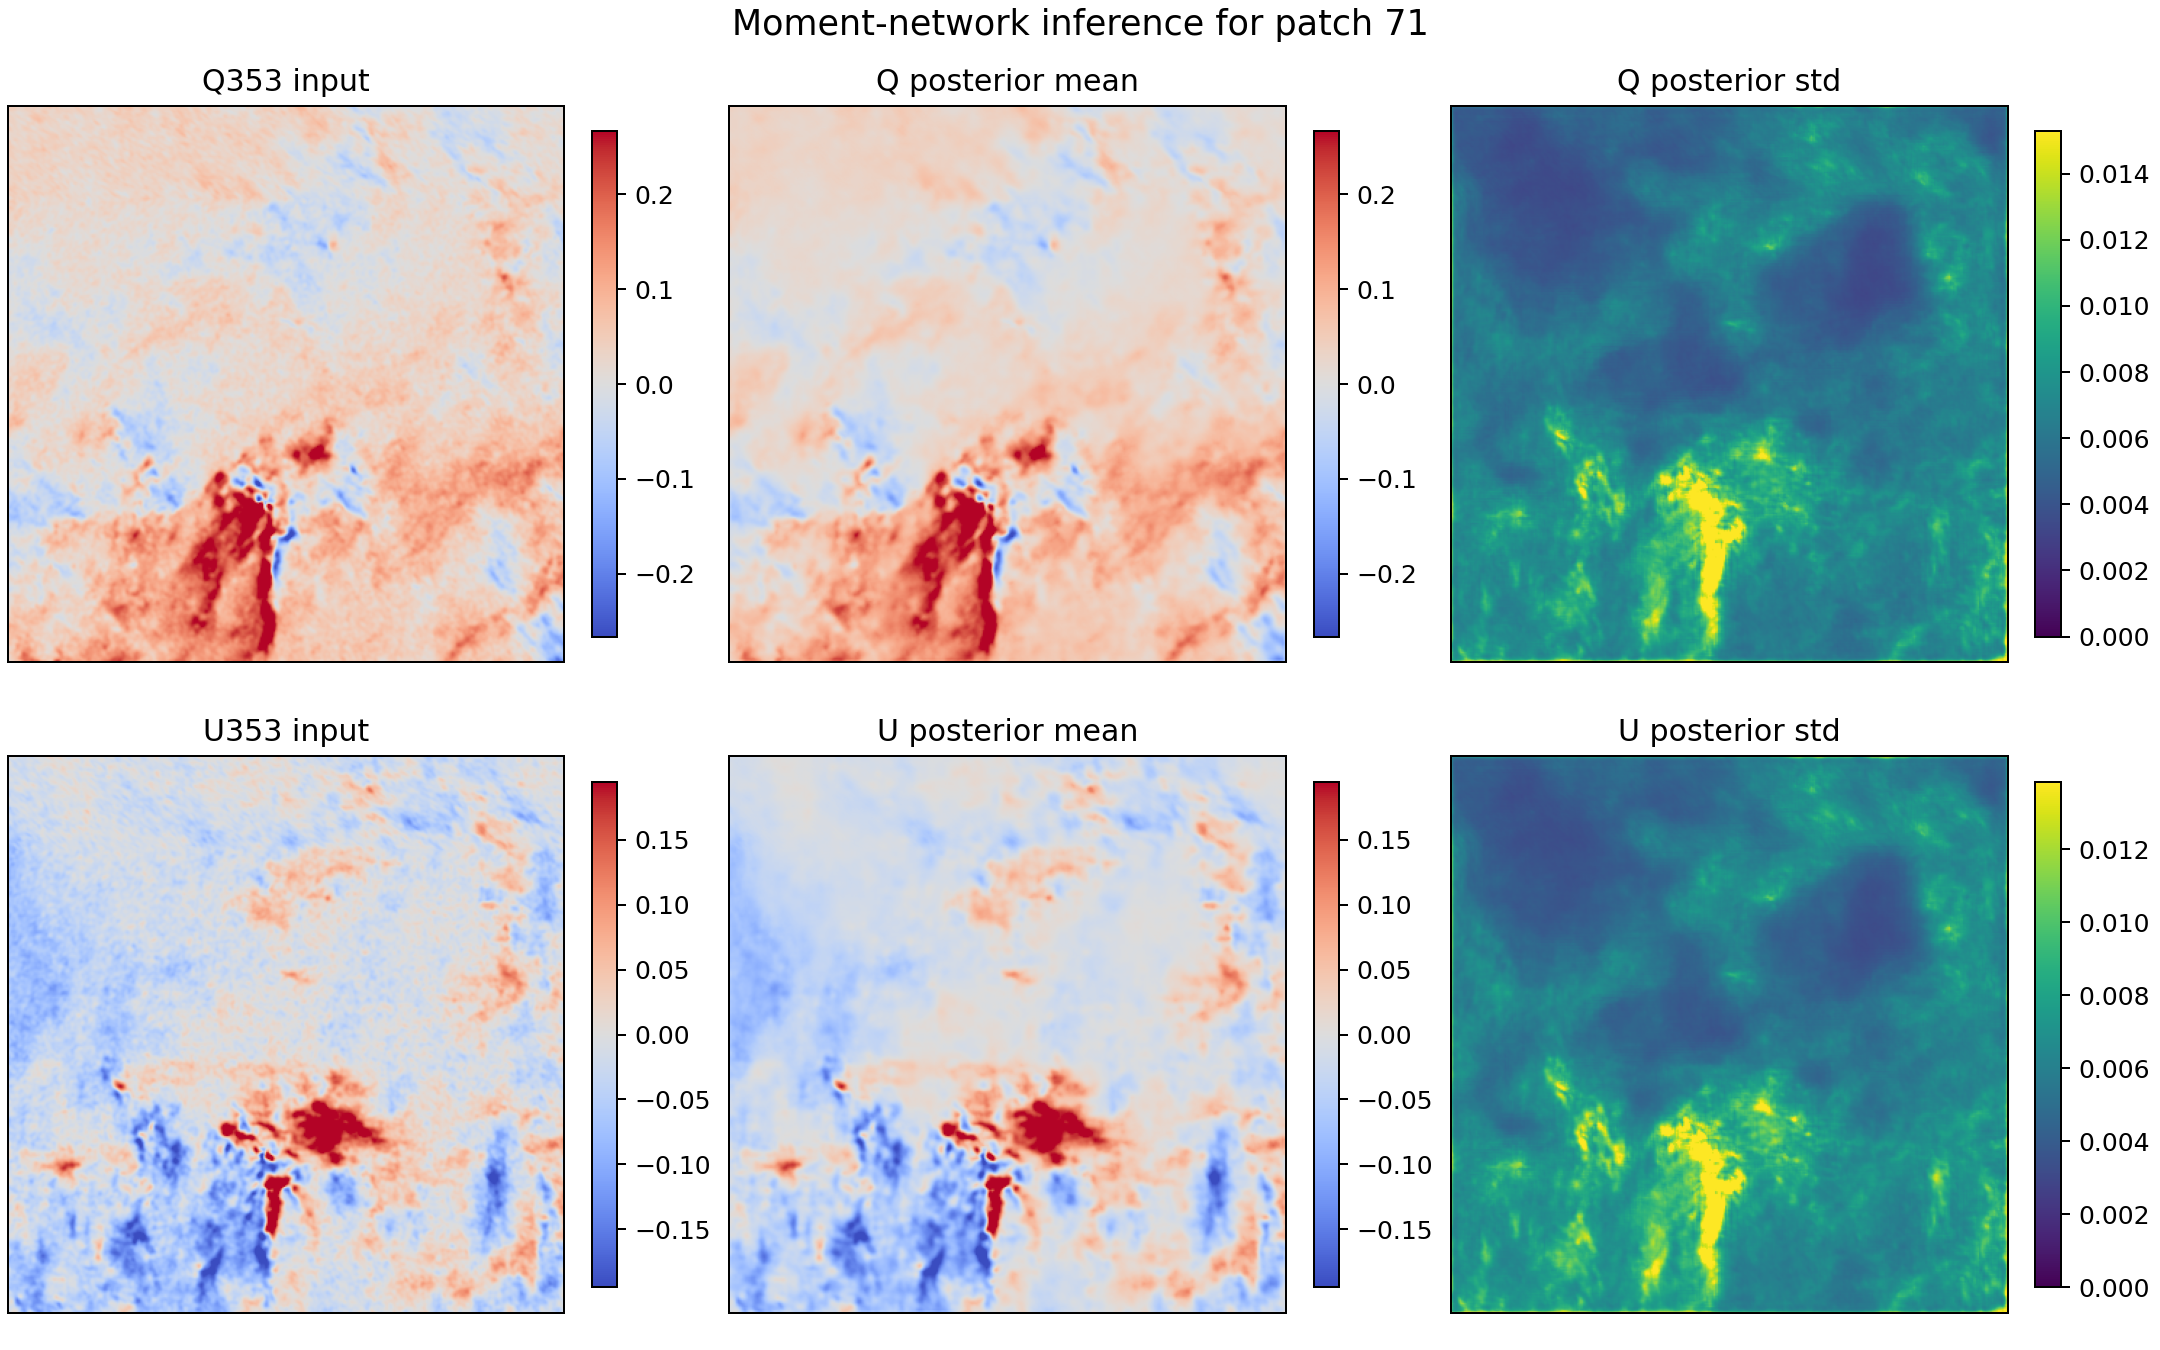
\includegraphics[height=0.72\textheight]{patch_71_moment_network_inference.png}

  \vspace{0.4em}
  \small
  These plots are visual baselines for the new Q/U/I two-stage run.
\end{frame}

\begin{frame}{Previous Version: More Examples}
  \centering
  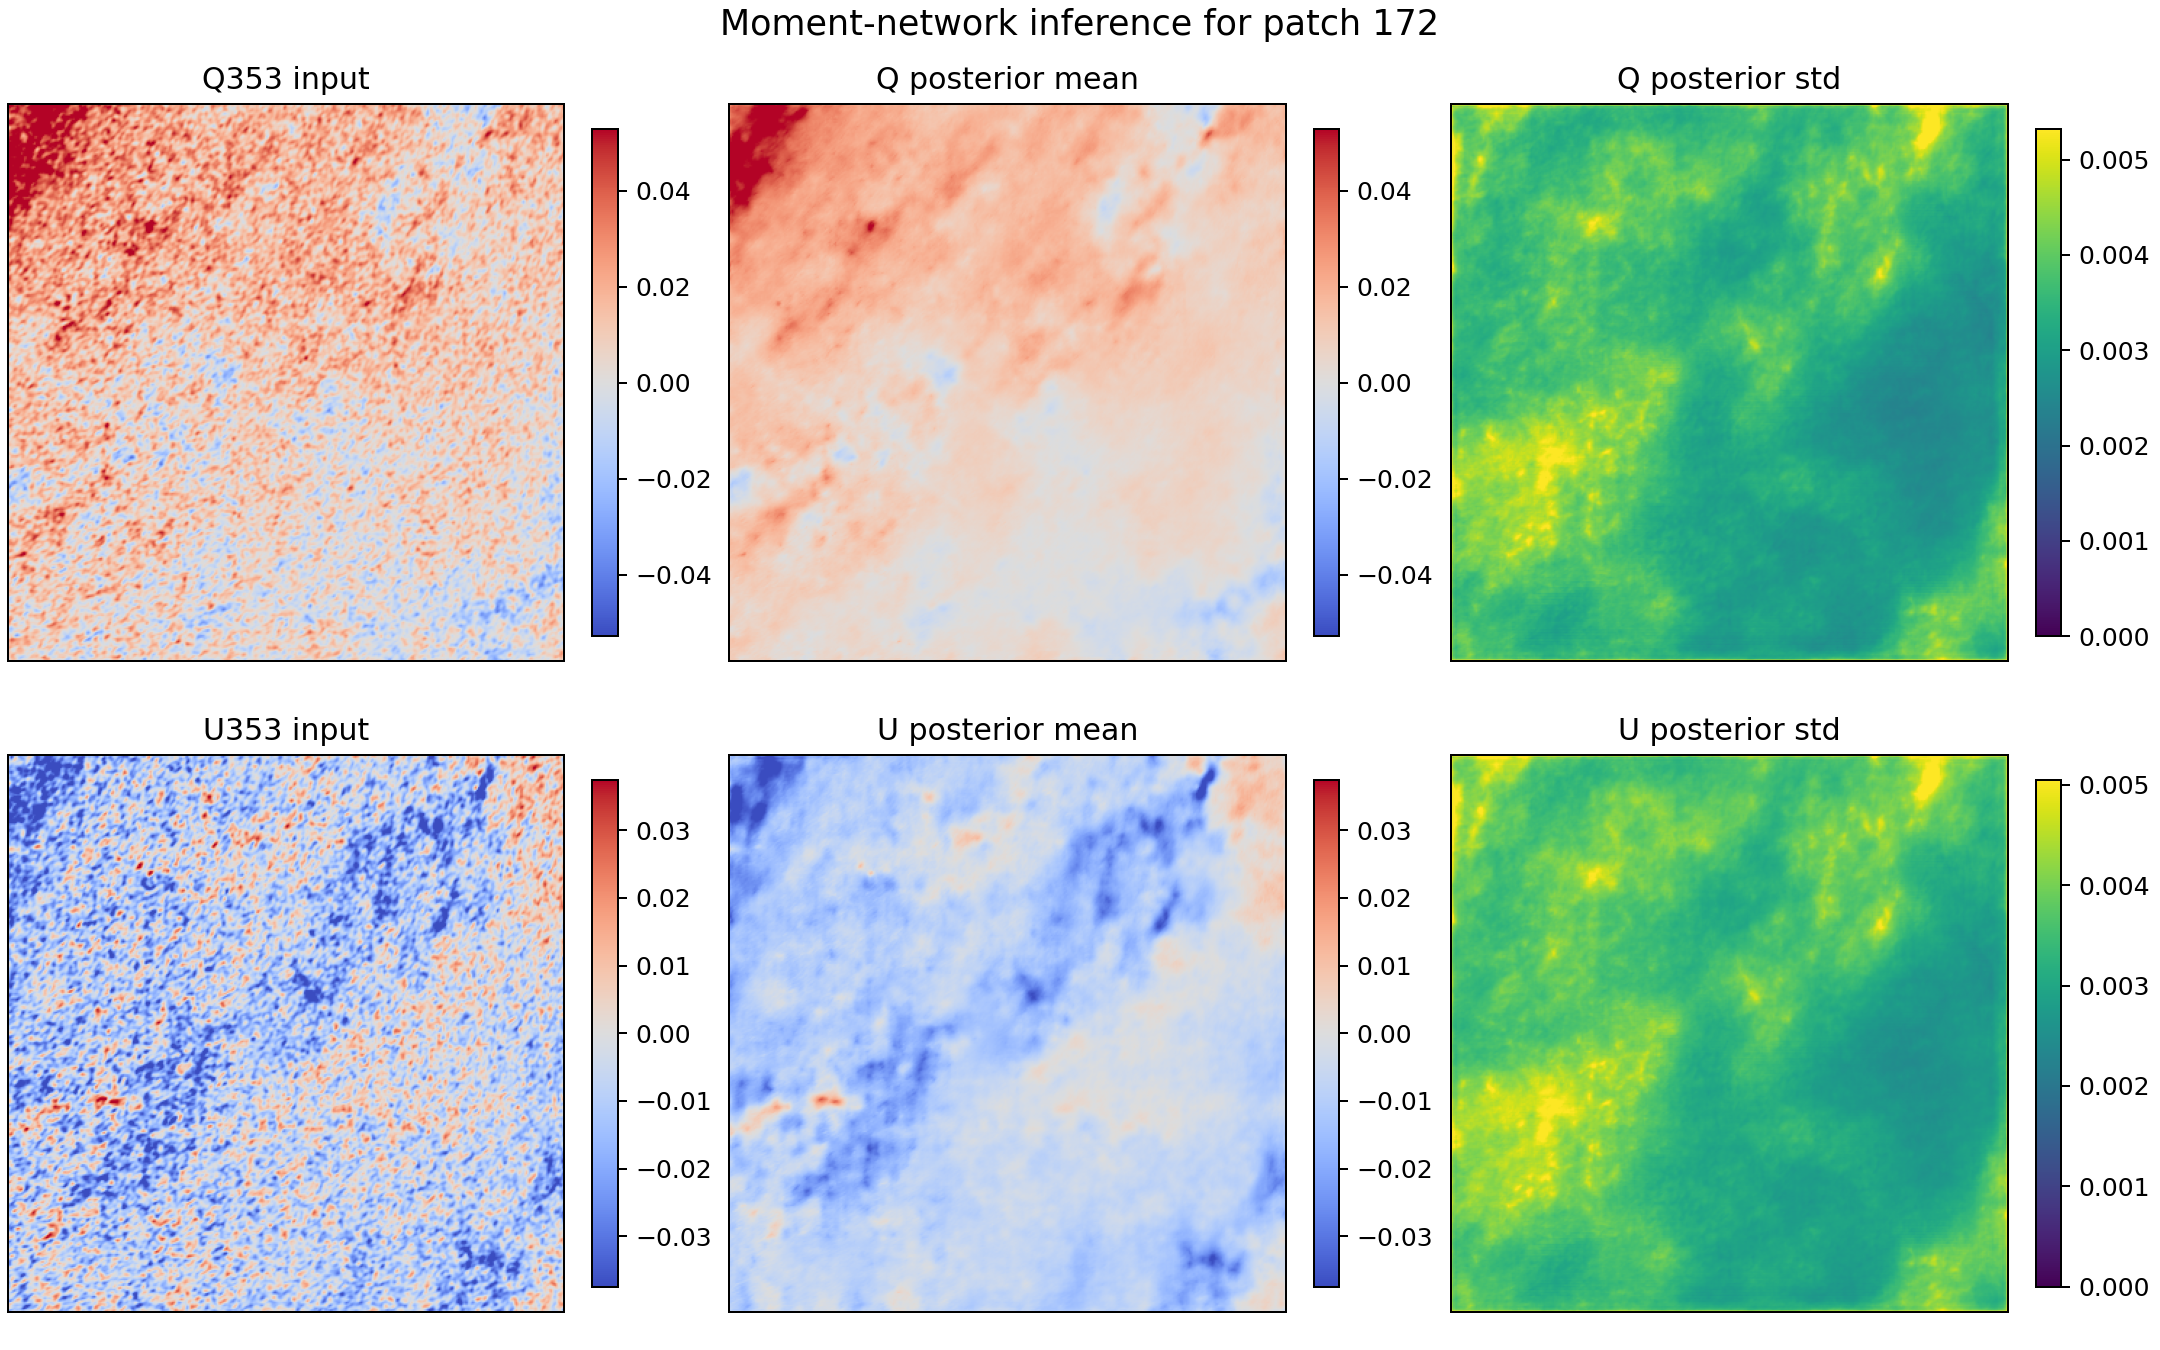
\includegraphics[height=0.72\textheight]{patch_172_moment_network_inference.png}

  \vspace{0.4em}
  \small
  After retraining, the same plotting script can compare the new two-stage uncertainty maps.
\end{frame}

\begin{frame}{Current Status}
  \begin{itemize}
    \item Dataset generation is complete for all patches.
    \item Previous joint-network results exposed a Q/U uncertainty coupling issue.
    \item The current training uses \(D=(d_Q,d_U,d_I)\), with \(I857\) as auxiliary data.
    \item The mean and variance are trained in two stages.
  \end{itemize}

  \vspace{0.7em}
  Main check after retraining:
  \[
    \sigma_Q(\data)
    \quad\text{and}\quad
    \sigma_U(\data)
  \]
  should no longer share an artificial common morphology.
\end{frame}

\end{document}
